\documentclass[hidelinks,11pt]{article}
\usepackage[utf8]{inputenc}
\usepackage{fullpage}
\usepackage{textcomp}
\usepackage{amsmath,amssymb}
\usepackage{setspace}
\usepackage[colorlinks=false]{hyperref}
\usepackage{textcomp} 
\usepackage{fancyhdr}
\usepackage[pdftex]{graphicx}
\usepackage{setspace}
\usepackage{listings}
\usepackage{appendix}
\usepackage[T1]{fontenc}
\usepackage{titlesec}
\usepackage{listings}
\usepackage{inconsolata}
\usepackage{color}
\graphicspath{ {./images/} }
\definecolor{gray}{rgb}{.98,.98,.98}
\lstset{frame=tb,
    language=C,                % choose the language of the code
    numbers=left,                   % where to put the line-numbers
    stepnumber=1,                   % the step between two line-numbers.        
    numbersep=5pt,                  % how far the line-numbers are from the code
    backgroundcolor=\color{gray},  % choose the background color. You must add \usepackage{color}
    showspaces=false,               % show spaces adding particular underscores
    showstringspaces=false,         % underline spaces within strings
    showtabs=false,                 % show tabs within strings adding particular underscores
    tabsize=4,                      % sets default tabsize to 2 spaces
    captionpos=b,                   % sets the caption-position to bottom
    breaklines=true,                % sets automatic line breaking
    breakatwhitespace=true,         % sets if automatic breaks should only happen at whitespace
    title=\lstname,
    frame=none,   
    belowskip=0pt,
    basicstyle=\ttfamily,
}
\renewcommand{\headrulewidth}{0pt}
\cfoot{\sc\thepage\ of \pageref{end}}

\begin{document}
\begin{titlepage} % Suppresses displaying the page number on the title page and the subsequent page counts as page 1

	\raggedleft % Right align the title page
	\rule{1pt}{\textheight} % Vertical line
	\hspace{0.05\textwidth} % Whitespace between the vertical line and title page text
	\parbox[b]{0.75\textwidth}{ % Paragraph box for holding the title page text, adjust the width to move the title page left or right on the page
        {\Huge\bfseries Algorithms and\\[0.5\baselineskip]Data Structures }\\[2\baselineskip] % Title
        
        {\large\textit{Notes on Algorithms, Data \\[0.5\baselineskip]Structures and other concepts}}\\[4\baselineskip] % Subtitle or further description
        
        {\Large\textsc{eric li}} % Author name, lower case for consistent small caps
        
        \vspace{0.5\textheight} % Whitespace between the title block and the publisher
        
        %{\noindent The Publisher~~\plogo}\\[\baselineskip] % Publisher and logo
        {\noindent\large\today}\\[\baselineskip]
    }
\end{titlepage}
\tableofcontents
\newpage
\section{Disclaimer}
The author(s) of this document assume(s) no responsibility or liability for any errors or omissions in the content of this document. The information contained in this site is provided on an “as is” basis with no guarantees of completeness, accuracy, usefulness or timeliness or of the results obtained from the use of this information.\\[0.5\baselineskip]
Information provided in this document has been taken from various sources and is by no means a comprehensive record of the source's views nor of the concepts represented.\\[1\baselineskip]
\textbf{Note:}\\
The concepts considered here will be largely captured in the scope of the language C, but can be generally be adapted to other languages, and are conceptually similar.
\section{Complexity}
There are three types of complexity:
\begin{itemize}
    \item Big-Omega ($\Omega$) (Best Case)
    \item Big-Theta ($\Theta$) (Average Case)
    \item Big-Oh ($O$) (Worst Case)
\end{itemize}
\textbf{Definition}\\
The worse case time complexity of an algorithm is a function that maps input sizes ($\mathbb N$) to the running times ($\mathbb R^+$).
\begin{figure}[h!]
    \centering
    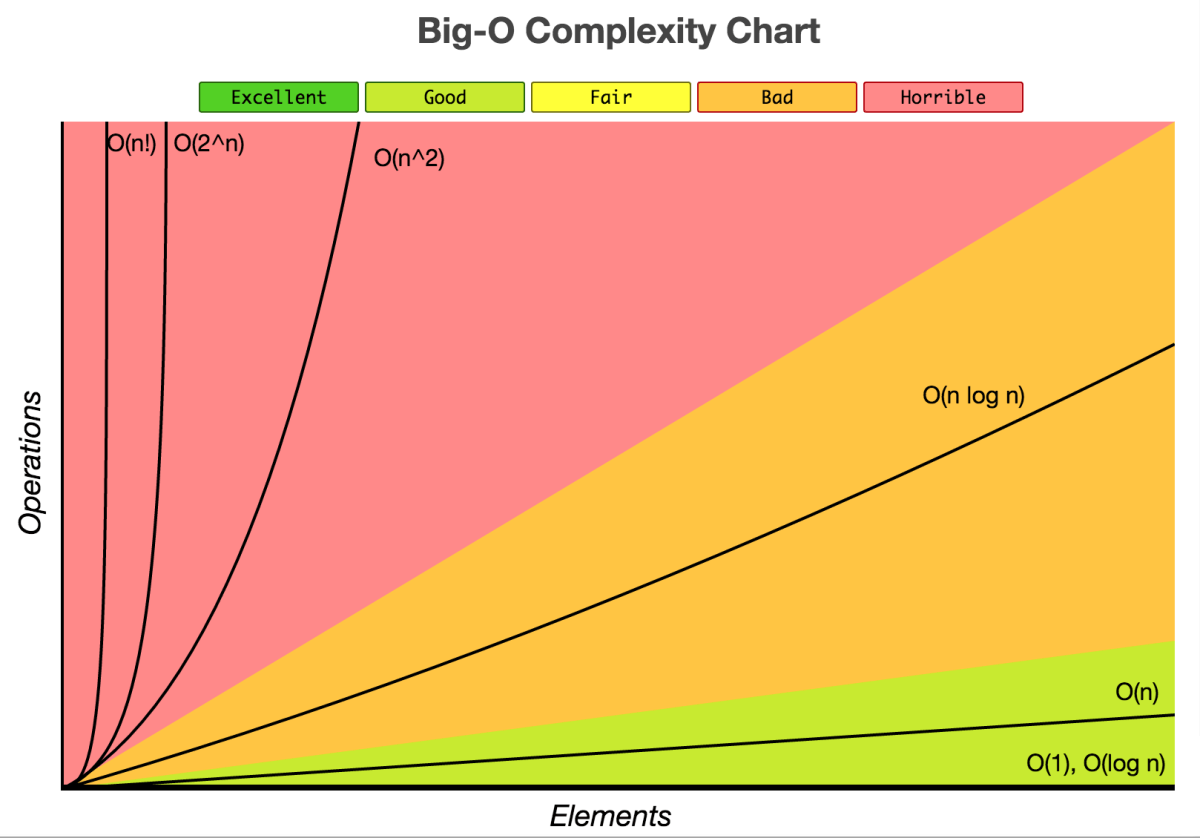
\includegraphics[scale=0.25]{complexity.png}
    \caption{Graph of Time Complexities}
\end{figure}\\[0.5\baselineskip]
\textbf{\textit{Note:}}\\
To find the Big-Oh of an algorithm we must determine a function that represents the worst possible running time of the algorithm for various sizes.
\subsection{Rules}
\begin{itemize}
    \item We are only interested in the "biggest function"
    \item We do not care about coefficients
\end{itemize}
\subsection{Examples}
\begin{itemize}
    \item $O(9n^2+6n+5) = O(9n^2) = O(n^2)$ 
    \begin{itemize}
        \item Since we are interested in only the biggest function (largest power) and no coefficients
    \end{itemize} 
    \item $O(n+\log n +5) = O(n)$ 
    \begin{itemize}
        \item We are interested in only the biggest function (largest power)
    \end{itemize} 
    \item $O(n\log) = O(n\log)$ \begin{itemize}
        \item Irreducible because it is a product of functions
    \end{itemize} 
    \item $O(7) = O(1)$
\end{itemize}
\subsection{How to find Big-Oh for code:}
\begin{itemize}
    \item Straight line code is $O(1)$ 
    \begin{itemize}
        \item "straight-line code" only runs once regardless of list size
    \end{itemize}
    \item For "if" statements, the Big-Oh is the biggest function of any case
    \item For "loops", the Big-Oh is the number of times that loop iterates multiplied by the Big-Oh of the inner code
\end{itemize}
Now the Big-Oh of the algorithm is the \textbf{most expensive} (simplified) function generated from the code.\\[.5\baselineskip]
\textbf{Example:}
\begin{lstlisting}
    int main(){
        int n = [user input]................\\O(1)
        int sum = 0;........................\\O(1)
        int i,j,k;..........................\\O(1)
        if (n==7){.........................\\O(1)
            return 1;.......................\\O(1)
        }
        else{ 
            for(i = 1;i<n;i*=2){............\\O(log n)
                for(j=n;j>0;j/=2){..........\\O(log n)
                    for(k=j;k<n;k+=2){......\\O(n)
                        sum +=(i+j+k);......\\O(1)
                    }
                }
            }
        }
    }
\end{lstlisting}
If we consider the $else$ block, we can multiply the worst case complexities and get $O(n(\log n)^2)$ from multiplying the outer for loop, the first nested, and the second nested loop, as well as the straight line code above.\\[0.5\baselineskip]
We do not consider the $if$ block since the $if$ block is not the worst case complexity.
\section{Linked Lists}
Linked lists are helpful in addressing some of the limitations that arrays face, such as inherent dynamic memory allocation and ease of modification. Instead of memory being assigned for use (as in the programming language C) linked lists are built on the premise of allocating memory as needed, and inserting or deleting as required by the user or data set.
\subsection{Structure}
A linked list is a linear data structure constructed from building blocks called nodes. Like other data structures, a node contains two items: data, which can be simple, compound, pointer, etc. and a memory address reference (or link to the next node, called a pointer in Figure 1). The address reference will access the next node's memory address in the list, and creates a `chain-like' relationship which will naturally produce a linear structure. There are two important nodes that are called the `head node' and the `tail node', which will influence operations and be explained in depth in the following sections.
\begin{figure}[h!]
    \centering
    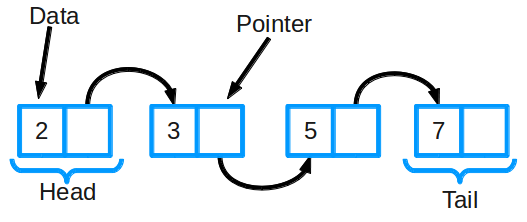
\includegraphics[scale=0.40]{linkedlist.png}
    \caption{Linked List}
\end{figure}
\subsection{Operations}
Linked lists support basic ADT operations of inserting, deleting, and modifying. For operations of inserting and deleting involving the head or tail, implementation requires several changes, but operates in a similar manner nonetheless.\\[0.5\baselineskip]
In order to understand operations on linked lists, we must identify what head pointers or head memory address are. Intuitively, the head address's are used to keep track of the linked list and allow for access on all functions. Without the head pointer, we lose the key to the linked list and are unable to both operate, and modify the list.\\[0.5\baselineskip] Therefore, it \textbf{imperative} that we return new head address's when modifications to the linked list occur that will affect it.
\subsubsection{Insertion}
Conceptually, inserting requires a list traversal to the desired point of insertion and memory address manipulation so that the address reference of the nodes link together appropriately.\\[0.5\baselineskip]
\textbf{Inserting in Linked Lists}\\
Inserting inside the list requires a few steps;
\begin{itemize}
    \item Traversal of the list to the desired location
    \item Accessing the previous node's reference to the succeeding node
    \item Setting the memory address of the succeeding node to the address link of the inserted node (linking inserted node to next node)
    \item Set the memory address of the inserted node to the address link of the previous node (linking inserted node with previous node)
    \item Return the new head address
\end{itemize}
Similarly, this can be adapted for \textbf{inserting at tail}.\\[.5 \baselineskip]
\textbf{Insertion at Head}\\
Inserting at the head of the list is by far the quickest insertion due to the lack of list traversal and ease of access to the head. Because of this, inserting at the head requires much fewer steps;
\begin{itemize}
    \item Access the head memory address
    \item Set the address to the memory link of the inserted node
    \item Set the head pointer to the inserted node's memory address(thereby setting the inserted node as the head)
    \item Return the new head address
\end{itemize}
As we can see, the steps are much more straight-forward and as such, if the items do not require a methodical order or specific location of insertion, inserting at the head is recommended.
\subsubsection{Deletion}
Conversely, we have deletion which follows a similar format as insertion of nodes;\\[0.5\baselineskip]
\textbf{Deleting in Linked Lists}\\
Deleting in linked lists requires several steps;
\begin{itemize}
    \item Traversal of the list to the desired node
    \item Accessing the previous node's reference to the node to delete
    \item Setting the previous node's reference to the node to delete's reference 
    \item Free the node to delete from memory
    \item Return the new head address
\end{itemize}
While this may be conceptually hard to grasp at first, when the implementation is shown, deleting will be much more clear and evident. Intuitively, we are aiming to delete the node, while allowing the previous node to preserve the connection with the succeeding nodes.\\[0.5\baselineskip]
\textbf{Deletion at Head}\\
With a basic understanding of deleting and inserting in a linked list, deleting at the head, is quite rudimentary;
\begin{itemize}
    \item Free the head node to delete it from memory
    \item Return the new head address
\end{itemize}

\section{Queues}
Queues are built heavily on concepts from linked lists and naturally, follows the same linear data structure. Queues provide a similar environment for "tail insertion" and "head deletion", which are appropriately named "enqueue" and "dequeue" respectively.
\section{Additional Notes}
The following sections are supplementary and cover topics that may not be considered algorithms and/or data structures but are interesting nonetheless.
\subsection{Variadic Functions}
Conventional functions, while effective and familiar, can be basic at times, and as such, C allows for variadic functions to handle the various parameter restrictions that conventional functions have.\\[0.5\baselineskip]
Variadic functions, as the name suggests, allows you to implement functions that take a variable number of arguments, and does this through a library in C. \\[0.5\baselineskip]
To add this library, we must call;
\begin{lstlisting}[belowskip=-1.80 \baselineskip]
    #include<stdarg.h>
\end{lstlisting}
\subsection{Macros}
To use variadic functions, we must use variadic functions macros to access and modify certain areas.
\begin{itemize}
    \item va\_list
    \item va\_start
    \item va\_arg
    \item va\_end
    \item va\_copy
\end{itemize}

\section{Sources}
https://www.cs.cmu.edu/~adamchik/15-121/lectures/Linked%20Lists/linked%20lists.html 
\\[0.5\baselineskip]
"Figure 1"\\
https://medium.com/@abdurrafeymasood/understanding-time-complexity-and-its-importance-in-technology-8279f72d1c6a
\\[0.5\baselineskip]
"Figure 2":\\
https://medium.com/@kenny.lin/singly-linked-lists-5cfdec60bea0
\\
\end{document}